\chapter{Réalisation}
\label{sec:quatriemechapitre}



\section{Introduction}
Dans ce chapitre nous exposons le travail achevé. Nous présentons en premier lieu l’architecture adapté pendant la réalisation du projet.\\ Ensuite, nous élaborons notre stack technologique choisi durant le développement de notre\\ système, tout en détaillant les outils utilisés pour développer notre application.\\ Nous clôturons ce chapitre par quelques captures d'écran traduisant le déroulement du plateforme.

\section{Architecture}
L’architecture à suivre dans notre projet est l’architecture MVC.\\
Le modèle-vue-contrôleur (en abrégé MVC, de l’anglais Model-View-Controller) est un modèle d'architecture de conception de logiciels qui permet de séparer les préoccupations de l'interface utilisateur, de la logique de l'application et des données. Le modèle est constitué de trois composants: le modèle, la vue et le contrôleur.


\begin{itemize}[label=$\bullet$]
    \item\textbf{Modèles(Model): } Ils représentent les données de l'application et contiennent la logique métier. Les modèles sont responsables de l'accès aux données, de leur manipulation et de leur persistance, généralement en interagissant avec une base de données ou d'autres sources de données.
    \vspace{4mm}
    \item\textbf{Vues(View): }Elles sont responsables de l'interface utilisateur et de l'affichage des données provenant des modèles. Les vues prennent les données fournies par les contrôleurs et les présentent de manière appropriée à l'utilisateur. Elles peuvent être des pages web, des éléments d'interface utilisateur, des rapports, etc.
    \vspace{4mm}
    \item\textbf{Contrôleurs(Controller) : }Ils reçoivent les entrées de l'utilisateur, interagissent avec les modèles pour effectuer les actions appropriées et sélectionnent la vue appropriée pour afficher les résultats au client. Les contrôleurs agissent essentiellement comme des intermédiaires entre les vues et les modèles, en traitant les requêtes de l'utilisateur et en coordonnant les interactions entre les différents composants de l'application.
\end{itemize}
\vspace{4mm}
\begin{figure}[H]
  \centering
  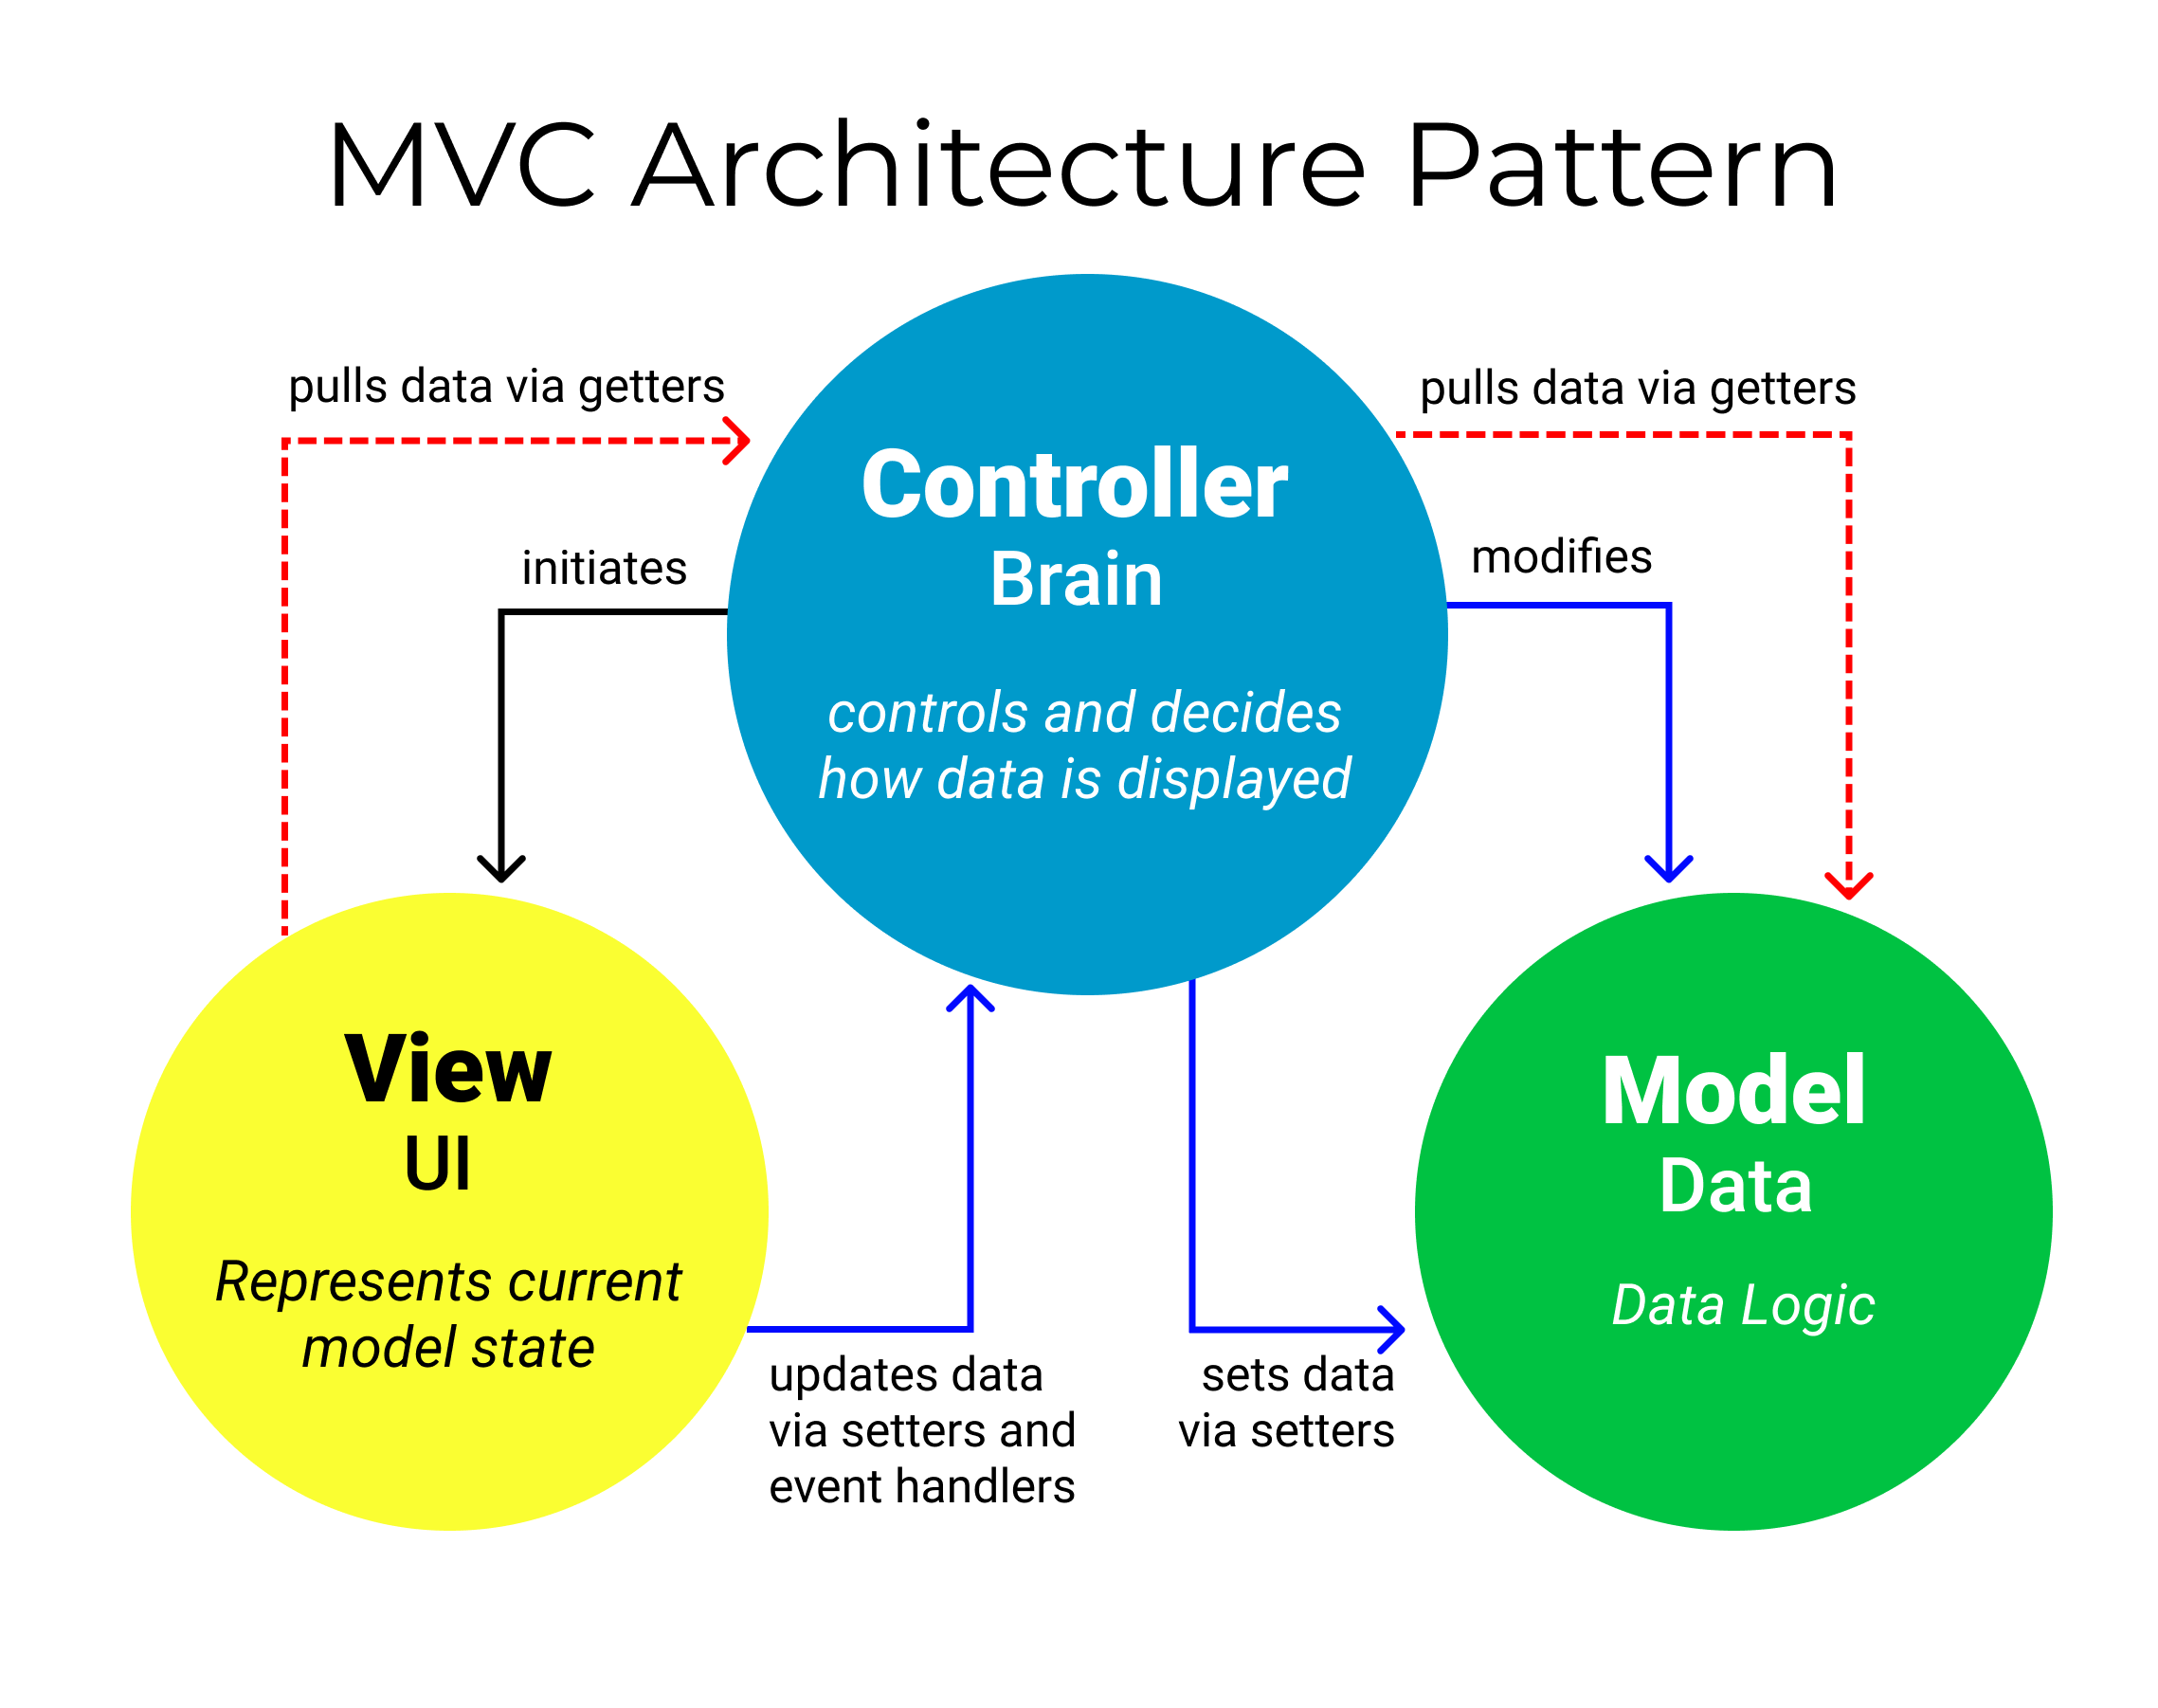
\includegraphics[scale=0.18]{cover/figuresChap4/MVC.png}
  \caption{Fonctionnement du modèle MVC }   
  \label{fig:picture}
\end{figure}




























\section{Environnement de développement}

Dans cette partie, nous décrivons les environnements logiciels et les technologies utilisées pour la réalisation de notre solution.
\vspace{5mm}

\subsection{Environnement technique}

\vspace{5mm}
\begin{itemize}[label=$\bullet$]
    \item \textbf{Vscode: } 
    \begin{figure}[H]
  \centering
  
\includegraphics[scale=0.75]{cover/figuresChap4/vscode.png}
  \caption{Logo de Vscode }   
  \label{fig:vscode}
\end{figure}
\vspace{4mm}
Visual Studio Code (voir figure \ref{fig:vscode}), conçu par Microsoft, est un éditeur de code léger et polyvalent. Il propose une gamme étendue de fonctionnalités, telles que la complétion intelligente du code, des outils de débogage avancés et une intégration fluide avec Git. Avec son interface conviviale et sa prise en charge multiplateforme, Visual Studio Code est largement plébiscité pour sa capacité à faciliter un codage efficace et collaboratif dans divers langages de programmation.\cite{vscode}
\vspace{4mm}
    \item \textbf{Overleaf:}
\begin{figure}[H]
  \centering
  
\includegraphics[scale=1.2]{cover/figuresChap4/overleaf (1).png}
  \caption{Logo de Overleaf }   
  \label{fig:overleaf}
\end{figure}
\vspace{4mm}
Overleaf (voir figure \ref{fig:overleaf}) est une plateforme de rédaction collaborative en ligne, spécialement conçue pour les documents LaTeX. Elle offre une multitude de fonctionnalités, notamment la compilation en temps réel, la gestion des versions, et la collaboration en temps réel. Avec une interface utilisateur intuitive et des outils de partage et de commentaires intégrés, Overleaf est devenu un choix privilégié pour la rédaction de documents académiques, scientifiques et techniques. Sa facilité d'utilisation et sa compatibilité multiplateforme en font une option populaire pour les équipes travaillant sur des projets de recherche et de rédaction collaborative.\cite{overleaf}
\vspace{4mm}
\item \textbf{Github:}
\begin{figure}[H]
  \centering
  
\includegraphics[scale=1.2]{cover/figuresChap4/github (1).png}
  \caption{Logo de Github }   
  \label{fig:github}
\end{figure}
\vspace{4mm}
GitHub (voir figure \ref{fig:github}) est une plateforme de développement logiciel collaborative, largement utilisée dans la communauté de la programmation. Fondée sur un système de contrôle de version basé sur Git, elle offre une multitude de fonctionnalités, notamment la gestion de projets, le suivi des problèmes, la collaboration entre développeurs et l'intégration continue. Avec son interface conviviale et ses outils avancés, GitHub facilite le développement et la collaboration sur des projets de logiciels open source et privés, en faisant un choix incontournable pour les équipes de développement modernes.\cite{github}
\newpage
\item \textbf{Lucidchart:}
\begin{figure}[H]
  \centering
  
\includegraphics[scale=0.33]{cover/figuresChap4/lucidchart-logo.png}
  \caption{Logo de Lucidchart }   
  \label{fig:lucidchart}
\end{figure}
Lucidchart (voir figure \ref{fig:lucidchart}) est une plateforme de création de diagrammes en ligne, offrant une multitude de fonctionnalités pour la visualisation de données et la conception de flux de travail. Développée par Lucid Software, cette application propose une interface intuitive et conviviale, permettant aux utilisateurs de créer facilement des diagrammes professionnels, des organigrammes, des cartes mentales, et bien plus encore. Avec ses outils de collaboration en temps réel, Lucidchart facilite le travail d'équipe et la communication visuelle, en permettant aux utilisateurs de partager et de commenter leurs créations en toute simplicité. Sa compatibilité multiplateforme et son intégration transparente avec d'autres outils en font un choix populaire pour la création et la gestion de diagrammes dans divers contextes professionnels et éducatifs.\cite{lucidchart}
\end{itemize}













\subsection{Environnement technique(AI)}
\begin{itemize}[label=$\bullet$]
\item\textbf{Python:}
\begin{figure}[H]
  \centering
  
\includegraphics[scale=0.1]{cover/figuresChap4/python.png}
  \caption{Logo de Python }   
  \label{fig:python}
\end{figure}
\vspace{4mm}
Python (voir figure \ref{fig:python}) est un langage de programmation polyvalent reconnu pour sa simplicité et sa lisibilité. Il est largement utilisé dans de nombreux domaines, notamment le développement web, l'automatisation de tâches, la science des données et l'intelligence artificielle. Sa syntaxe claire et concise en fait un choix idéal pour les débutants et les professionnels. Python est particulièrement prisé dans le domaine de l'intelligence artificielle en raison de sa riche bibliothèque d'outils et de frameworks spécialisés. Ces ressources puissantes permettent aux développeurs d'implémenter des algorithmes d'apprentissage automatique, de traitement du langage naturel et de vision par ordinateur avec une relative facilité. Ainsi, Python se distingue comme un langage incontournable pour ceux qui souhaitent explorer et exploiter les vastes possibilités de l'intelligence artificielle.\cite{python}
\vspace{4mm}
\item\textbf{NumPy:}
\begin{figure}[H]
  \centering
  
\includegraphics[scale=0.1]{cover/figuresChap4/NumPy.png}
  \caption{Logo de NumPy }   
  \label{fig:numpy}
\end{figure}
\vspace{4mm}
NumPy (voir figure \ref{fig:numpy}) est une bibliothèque Python pour le calcul scientifique qui prend en charge de grands tableaux et matrices multidimensionnels, ainsi qu'un ensemble de fonctions mathématiques pour fonctionner efficacement sur ces tableaux et matrices.\cite{numpy}
\vspace{4mm}
\item\textbf{NLTK:}
\begin{figure}[H]
  \centering
  
\includegraphics[scale=0.15]{cover/figuresChap4/NLTK.png}
  \caption{Logo de NLTK }   
  \label{fig:nltk}
\end{figure}
\vspace{4mm}
NLTK (voir figure \ref{fig:nltk}) est une bibliothèque Python qui fournit un ensemble d'outils et de ressources pour les tâches de traitement du langage naturel. Elle offre des divers fonctionnalités et algorithmes pour des tâches telles que la tokenisation, la racinisation (stemming), le marquage (tagging), l'analyse (parsing), le raisonnement sémantique, etc. NLTK est largement utilisé dans le domaine de traitement du language naturel pour la recherche et l'éducation.\cite{nltk}
\vspace{4mm}
\item\textbf{Scikit-learn:}
\begin{figure}[H]
  \centering
  
\includegraphics[scale=0.08]{cover/figuresChap4/Scikit_learn.png}
  \caption{Logo de Scikit-learn}   
  \label{fig:sklearn}
\end{figure}
\vspace{4mm}
Scikit-learn (voir figure \ref{fig:sklearn}) est une bibliothèque Python destinée à l'apprentissage automatique.Elle propose dans son framework de nombreuses bibliothèques d’algorithmes à implémenter, clé en main.Elle comprend notamment des fonctions pour estimer des forêts aléatoires, des régressions logistiques, des algorithmes de classification, et les machines à vecteurs de support. Elle est conçue pour s'harmoniser avec d'autres bibliothèques Python, notamment NumPy et SciPy.\cite{sklearn}
\end{itemize}









\subsection{Choix technologiques}
\vspace{5mm}
\subsubsection{La partie Frontend}
\vspace{5mm}
Dans le domaine du développement web, l'interface désigne la partie visible d'un site web ou d'une application avec laquelle les utilisateurs interagissent directement. Elle englobe la présentation, la structure et les fonctionnalités de l'interface utilisateur, ainsi que les technologies et les langages utilisés pour sa conception. Le développement frontal implique généralement l'utilisation de HTML pour structurer le contenu, de CSS pour le style et la mise en page, et de JavaScript pour rendre les éléments interactifs et gérer leur comportement. Afin d’élaborer notre interface web, nous
avons utilisé :
\begin{itemize}[label=$\bullet$]
\begin{figure}[H]
  \centering
  
\includegraphics[scale=0.5]{cover/figuresChap4/react js.png}
  \caption{Logo de React}   
  \label{fig:react}
\end{figure}
  \item \textbf{React :}React (voir figure \ref{fig:react}) est une bibliothèque JavaScript open-source pour la construction d'interfaces utilisateur. Elle fournit une approche déclarative et efficace pour construire des applications web complexes et interactives. React utilise une architecture basée sur des composants, où les éléments de l'interface utilisateur sont décomposés en composants réutilisables et autonomes. Il utilise un DOM (Document Object Model) virtuel qui optimise les performances de rendu en ne mettant à jour que les parties nécessaires de l'interface utilisateur. Le flux de données unidirectionnel et l'algorithme de diffing efficace de React le rendent très performant dans le traitement des mises à jour et la gestion des changements d'état.\cite{react}
\end{itemize}





\vspace{5mm}
\subsection{Environnement matériel}
\vspace{5mm}
Le travail a été réalisé sur un ordinateur portable qui dispose les caractéristiques suivantes:
\vspace{4mm}
\begin{itemize}[label=$\bullet$]
    \item\textbf {Processeur:} Intel(R) Core(TM) i5-10500H CPU.
    \vspace{3mm}
    \item\textbf {Mémoire vive:} 16 GB.
    \vspace{3mm}
    \item\textbf {Disque dur:} 512 GB.
\end{itemize}

\section{Présentation des interfaces du plateforme}
Dans cette section, nous allons présenter quelques interfaces de notre application \\ pour visualiser certains cas d’utilisation.
\newpage
\subsection{Interface de login }
La figure (voir la figure \ref{fig:signin} )  indique l’interface d’authentification ou l’utilisateur entre ses données d’identification
correctement afin d’accéder aux autres fonctionnalités de l’application.

\begin{figure}[H]
  \centering
  
\includegraphics[scale=0.8]{chapitre4/interfaces/signinfina.PNG}
  \caption{Interface d’authentification}   
  \label{fig:signin}
\end{figure}
\vspace{5mm}
\subsection{Interface d'accueil }
\vspace{5mm}
L'interface d'accueil (voir la figure \ref{fig:accueil1}) offre une vue d'ensemble complète des tâches et des problèmes en cours. La première partie affiche les tâches dues, en retard, incomplètes et terminées, tandis que la seconde partie (voir la figure \ref{fig:accueil2} ) présente une répartition des tâches par section ainsi qu'un calendrier des événements à venir.
\vspace{8mm}
\begin{figure}[H]
  \centering
  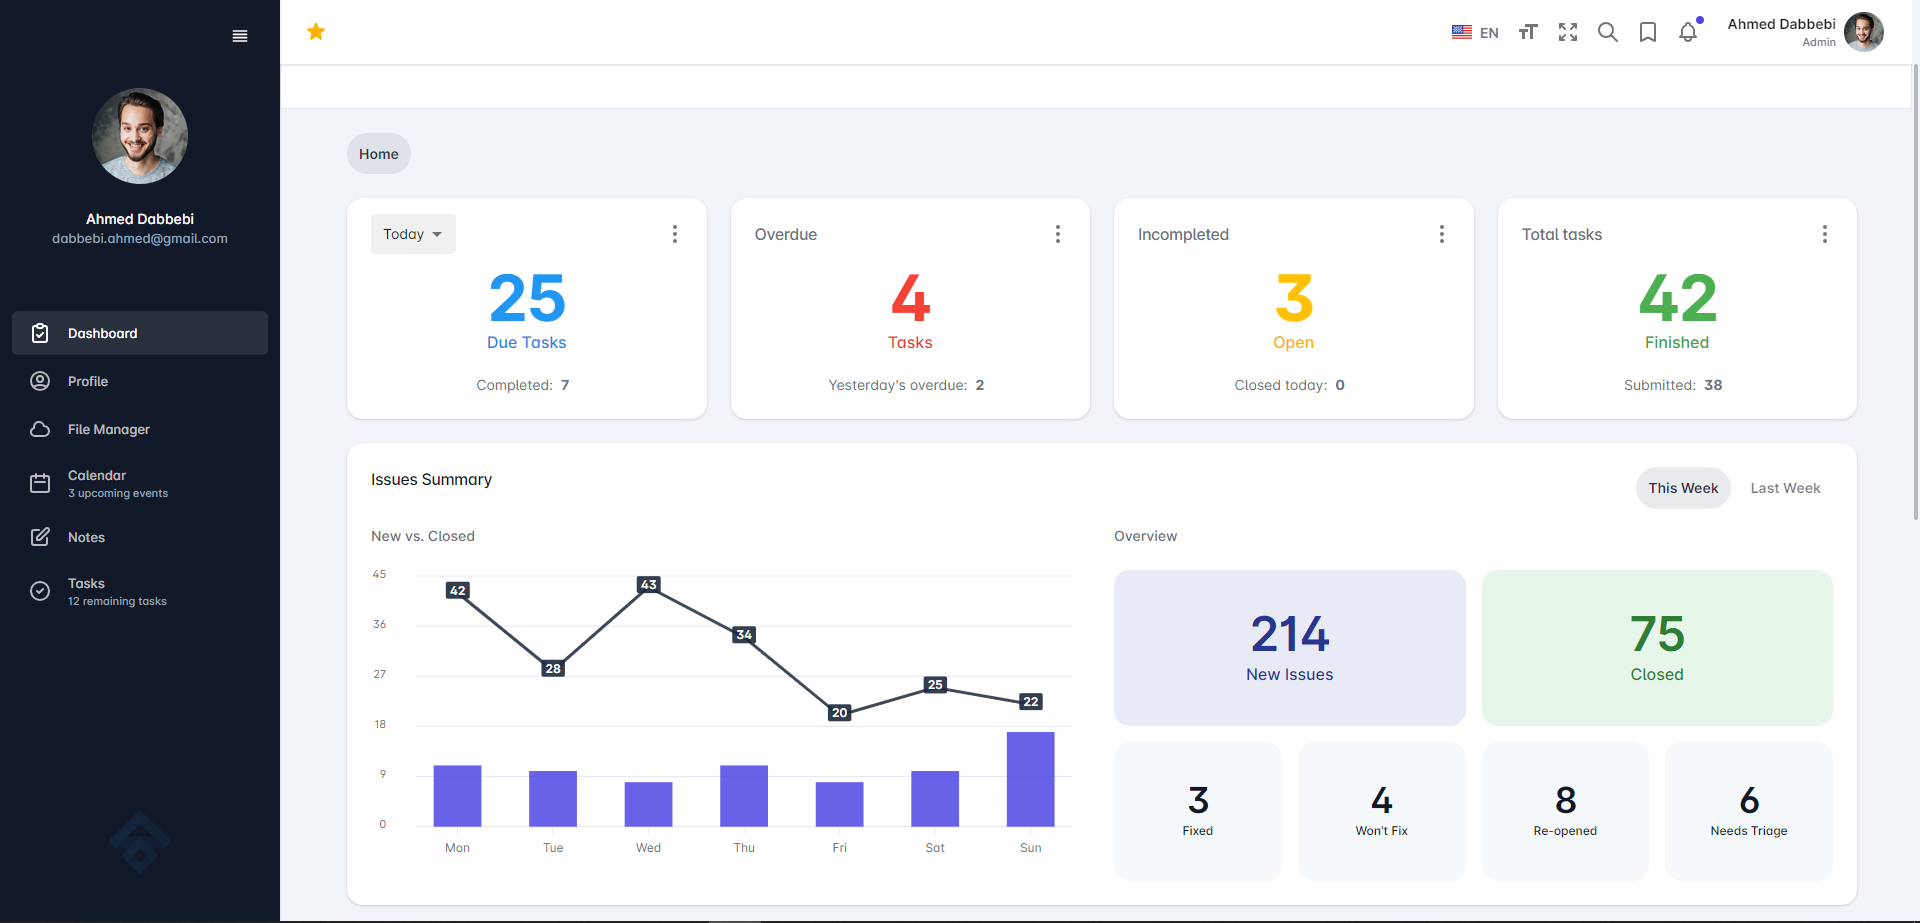
\includegraphics[scale=0.45]{chapitre4/interfaces/dashboard1.PNG}
  \caption{Interface d’accueil (1)}   
  \label{fig:accueil1}
\end{figure}
\begin{figure}[H]
  \centering
  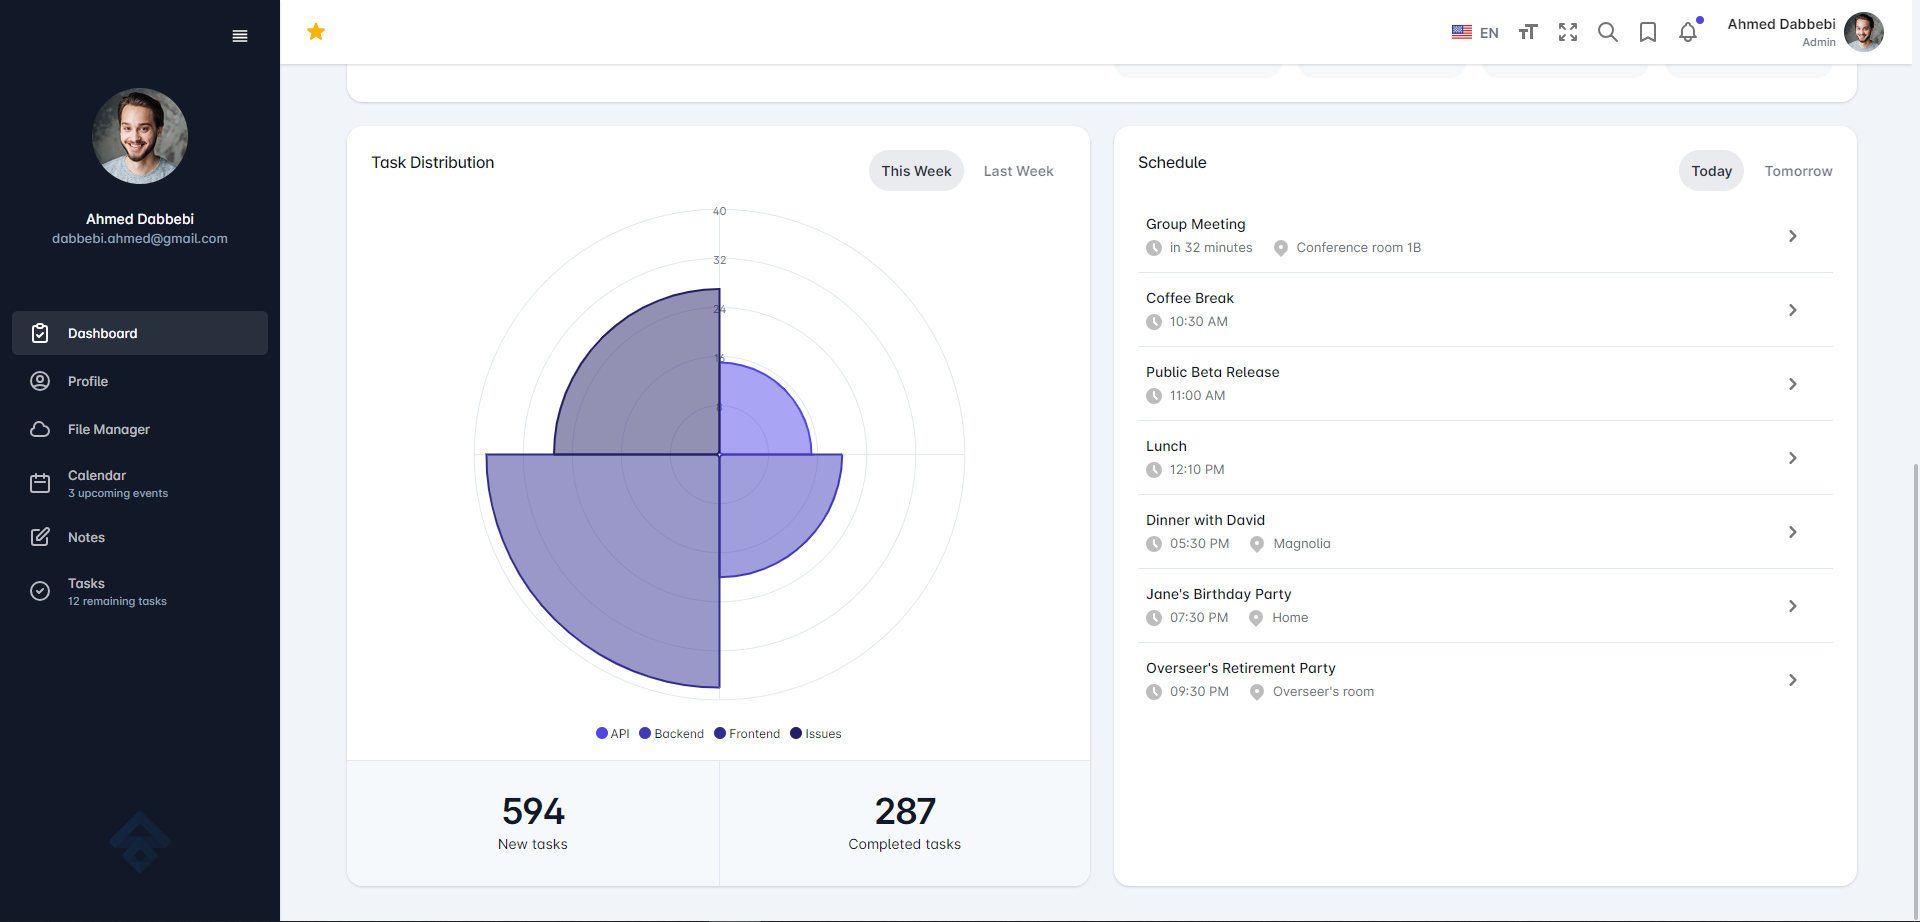
\includegraphics[scale=0.45]{chapitre4/interfaces/dashboard2.PNG}
  \caption{Interface d’accueil (2)}   
  \label{fig:accueil2}
\end{figure}

\vspace{5mm}
\subsection{Interface de gestionnaire de fichiers }
\vspace{5mm}
L'interface de gestionnaire de fichiers (voir la figure \ref{fig:filemanag} )  permet aux étudiants de gérer efficacement leurs documents et ressources numériques (voir la figure \ref{fig:file} ). Elle offre des fonctionnalités d'organisation (voir la figure \ref{fig:folder} ) et de visualisation des fichiers, facilitant ainsi la gestion de contenu.

\begin{figure}[H]
  \centering
  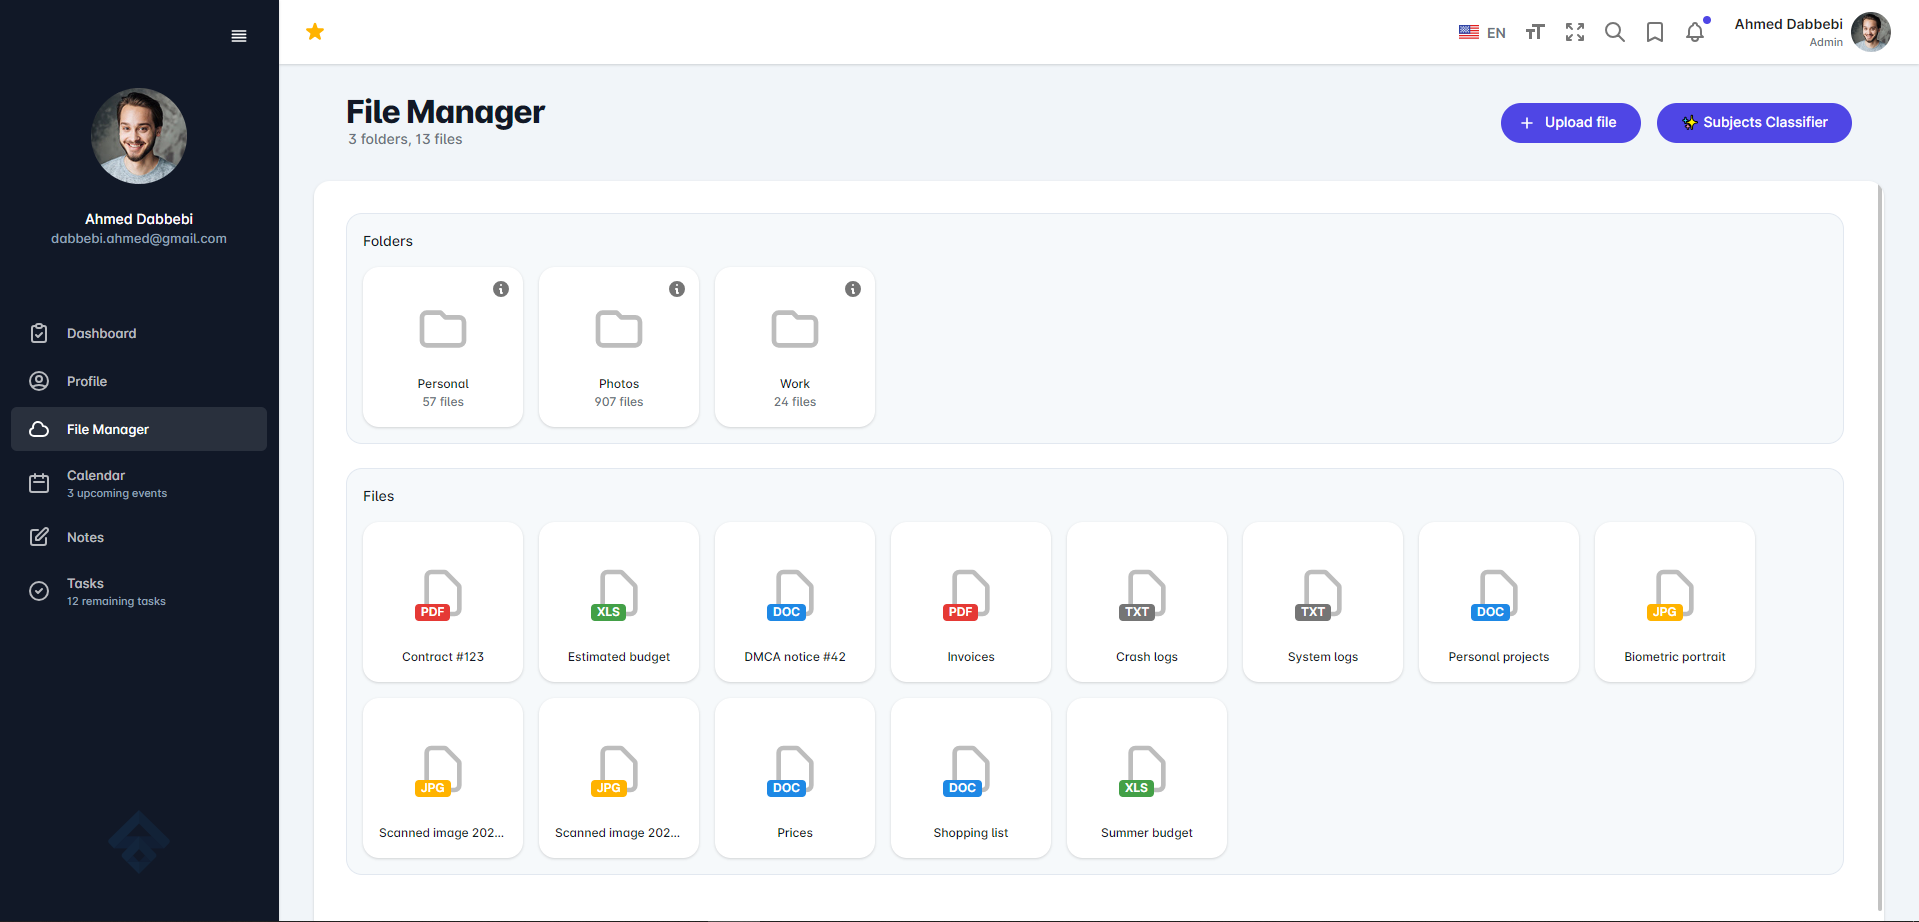
\includegraphics[scale=0.45]{chapitre4/interfaces/file manager.PNG}
  \caption{Interface de gestionnaire de fichiers}   
  \label{fig:filemanag}
\end{figure}
\begin{figure}[H]
  \centering
  
\includegraphics[scale=0.68]{chapitre4/interfaces/file.PNG}
  \caption{Interface de fichier}   
  \label{fig:file}
\end{figure}
\begin{figure}[H]
  \centering
  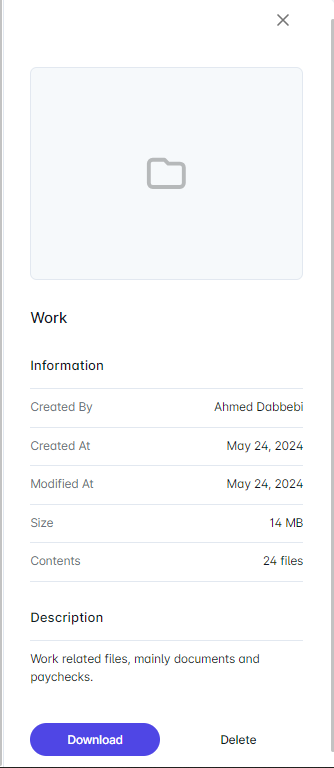
\includegraphics[scale=0.7]{chapitre4/interfaces/folder.PNG}
  \caption{Interface de dossier}   
  \label{fig:folder}
\end{figure}

\vspace{5mm}
\subsection{Interface de calendrier }
\vspace{5mm}
L'interface de calendrier (voir la figure \ref{fig:calendar}) permet aux étudiants d'ajouter (voir la figure \ref{fig:addevent}) et de visualiser des événements étiquetés (voir la figure \ref{fig:editlabelcal}). Grâce à une vue intuitive et interactive, les étudiants peuvent facilement organiser leurs événements et rendez-vous en les catégorisant par étiquettes.
\begin{figure}[H]
  \centering
  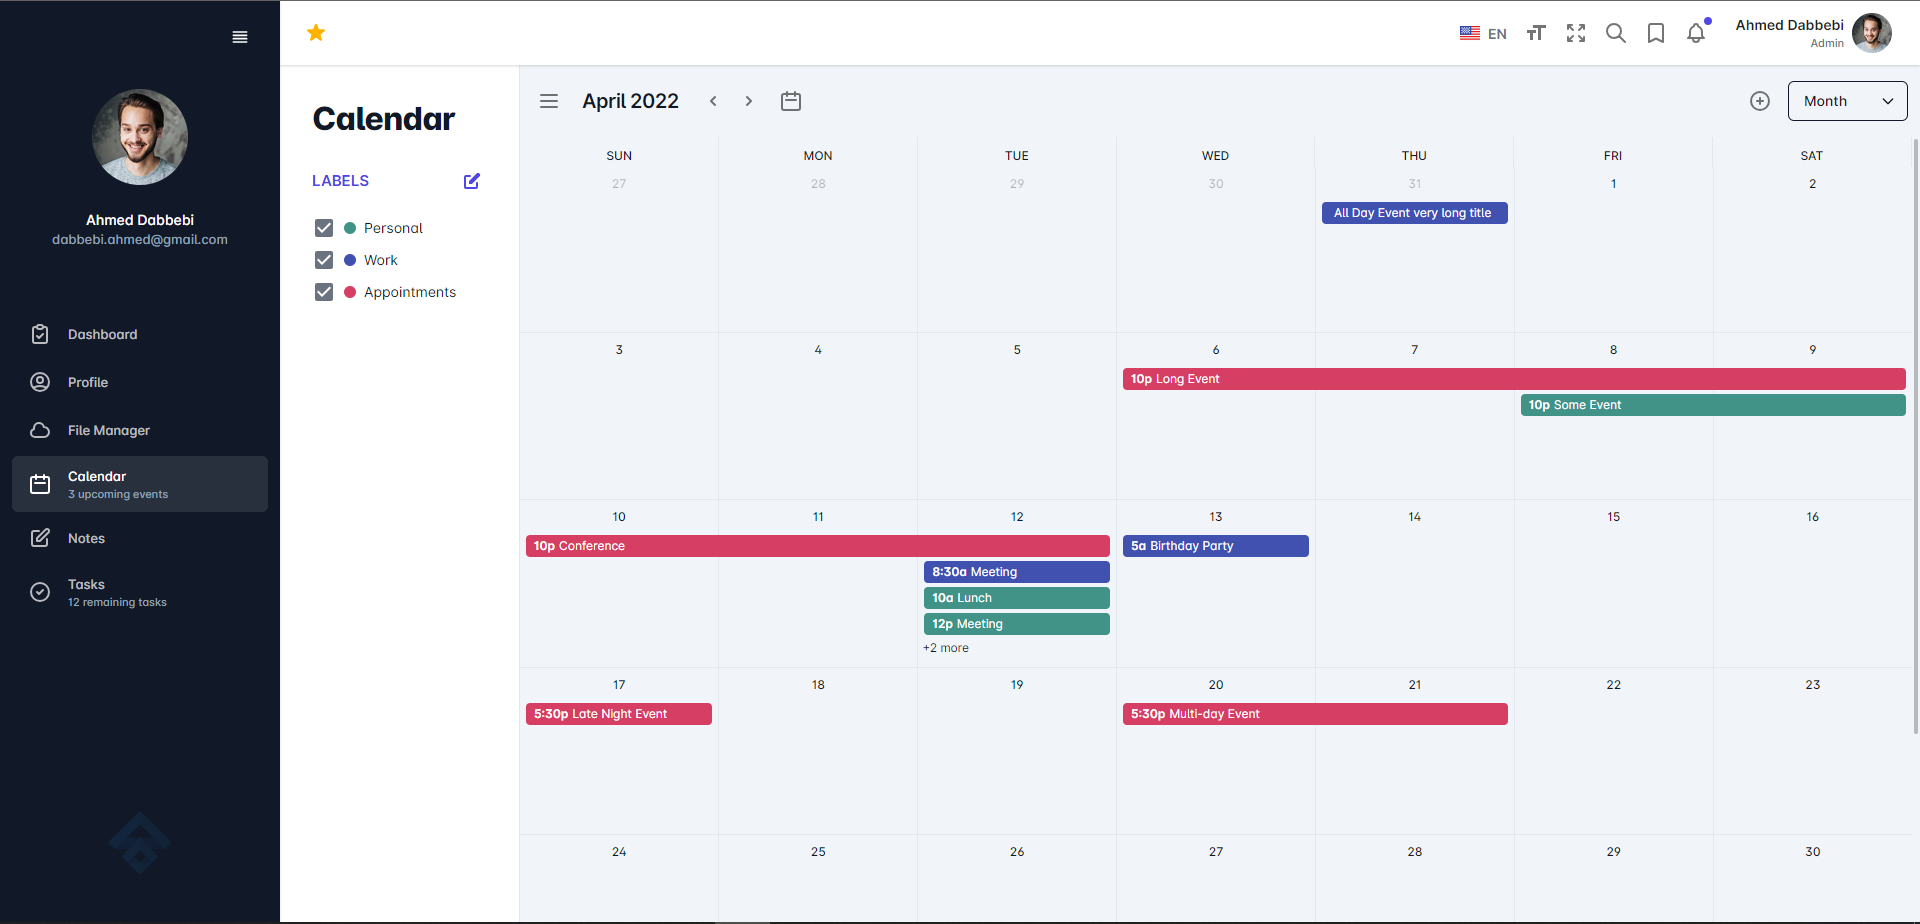
\includegraphics[scale=0.45]{chapitre4/interfaces/calendar.PNG}
  \caption{Interface de calendrier}   
  \label{fig:calendar}
\end{figure}
\begin{figure}[H]
  \centering
  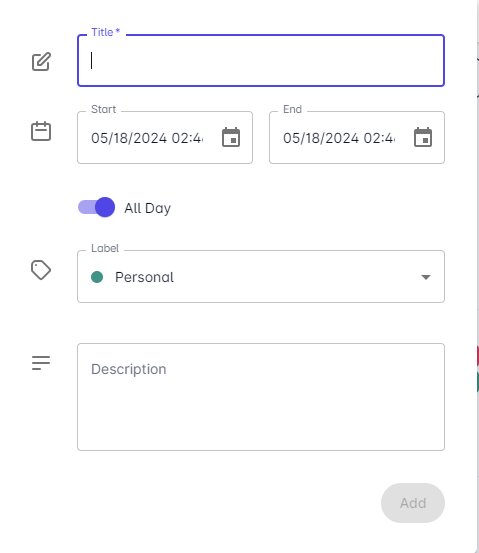
\includegraphics[scale=0.7]{chapitre4/interfaces/add event.PNG}
  \caption{Interface d'ajout d'un nouveau événement}   
  \label{fig:addevent}
\end{figure}
\begin{figure}[H]
  \centering
  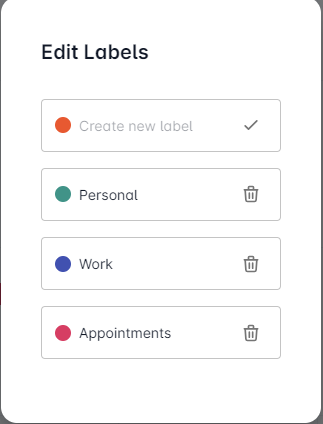
\includegraphics[scale=0.7]{chapitre4/interfaces/edit label calendar.PNG}
  \caption{Interface de modification de labels}   
  \label{fig:editlabelcal}
\end{figure}

\vspace{5mm}
\subsection{Interface de notes }
\vspace{5mm}
L'interface de note (voir la figure \ref{fig:notesinter}) offre la possibilité d'ajouter (voir la figure \ref{fig:addnote}) des notes personnalisées et de leur associer des rappels. Cette fonctionnalité aide les étudiants à gérer leurs idées et remarques importantes tout en garantissant qu'aucune échéance n'est oubliée grâce aux notifications de rappel.
\begin{figure}[H]
  \centering
  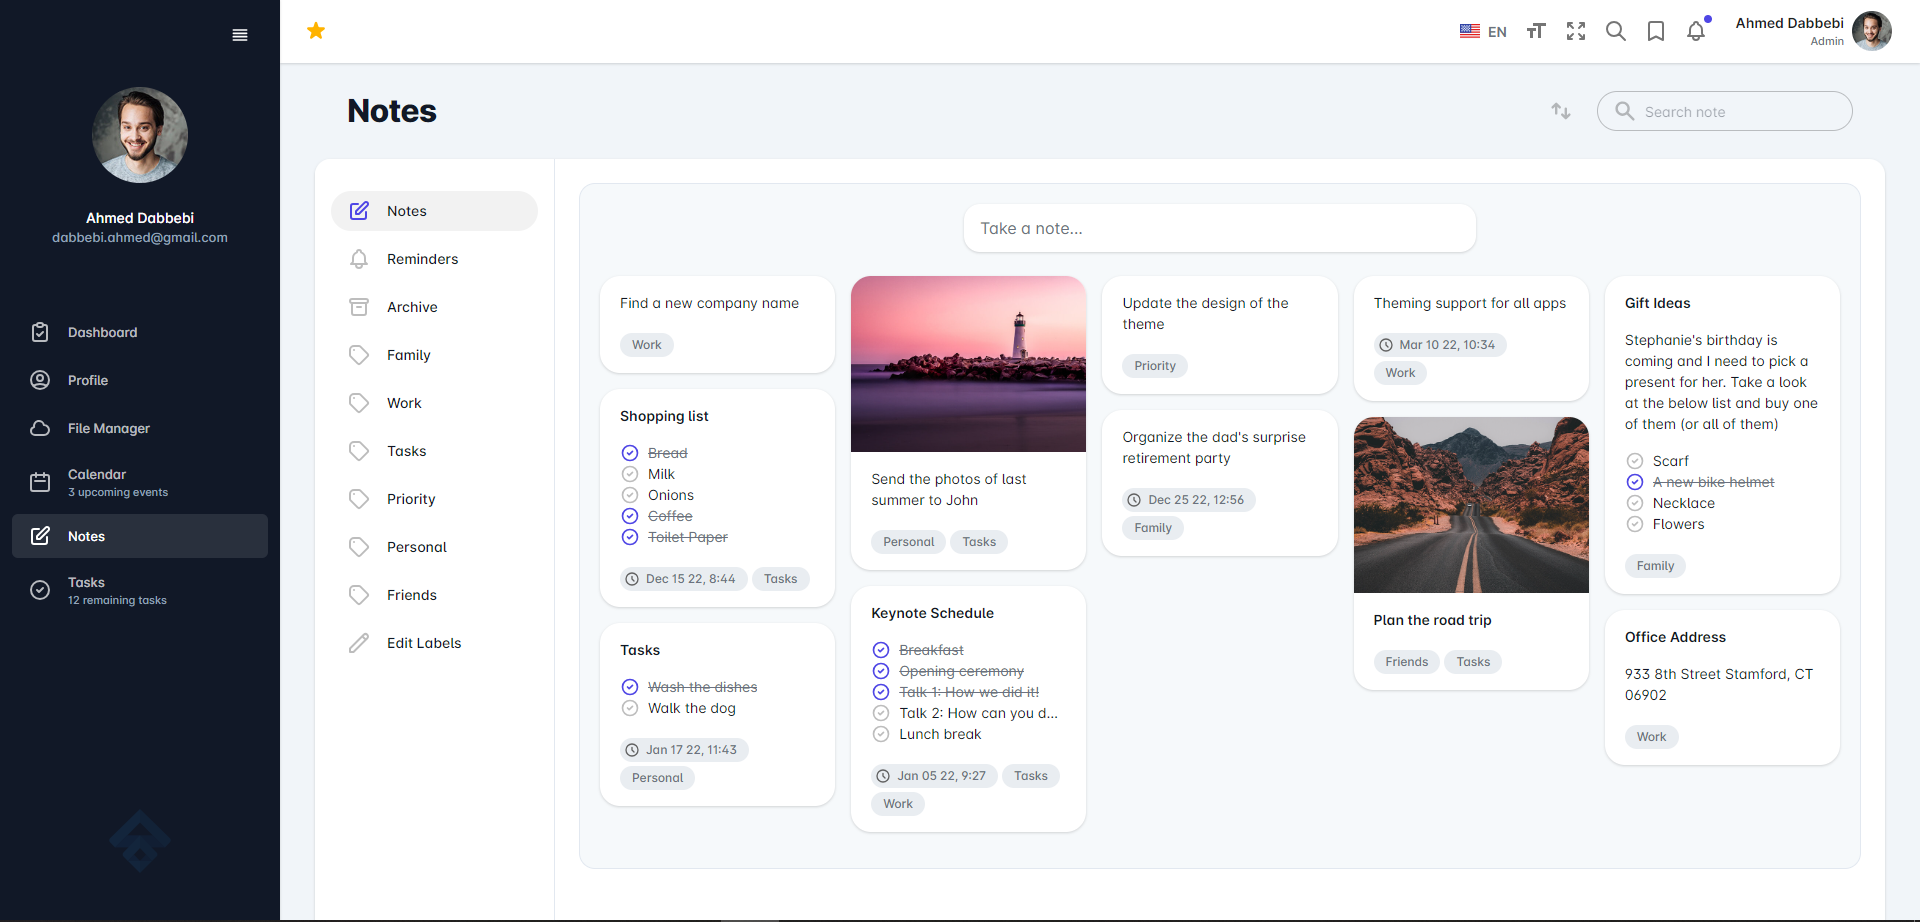
\includegraphics[scale=0.45]{chapitre4/interfaces/notes.PNG}
  \caption{Interface de notes}   
  \label{fig:notesinter}
\end{figure}
\begin{figure}[H]
  \centering
  
\includegraphics[scale=0.8]{chapitre4/interfaces/add note.PNG}
  \caption{Interface d'ajout d'une nouvelle note}   
  \label{fig:addnote}
\end{figure}

\vspace{5mm}
\subsection{Interface de tâches }
\vspace{5mm}
L'interface de tâches (voir la figure \ref{fig:taches}) permet aux étudiants d'ajouter (voir la figure \ref{fig:addtask}) des tâches en spécifiant leur niveau de priorité (faible, normal, élevée) et de les regrouper par section (voir la figure \ref{fig:addsection}). Cette organisation facilite la gestion des activités quotidiennes en assurant que les tâches les plus urgentes et importantes sont clairement identifiées et bien structurées.
\begin{figure}[H]
  \centering
  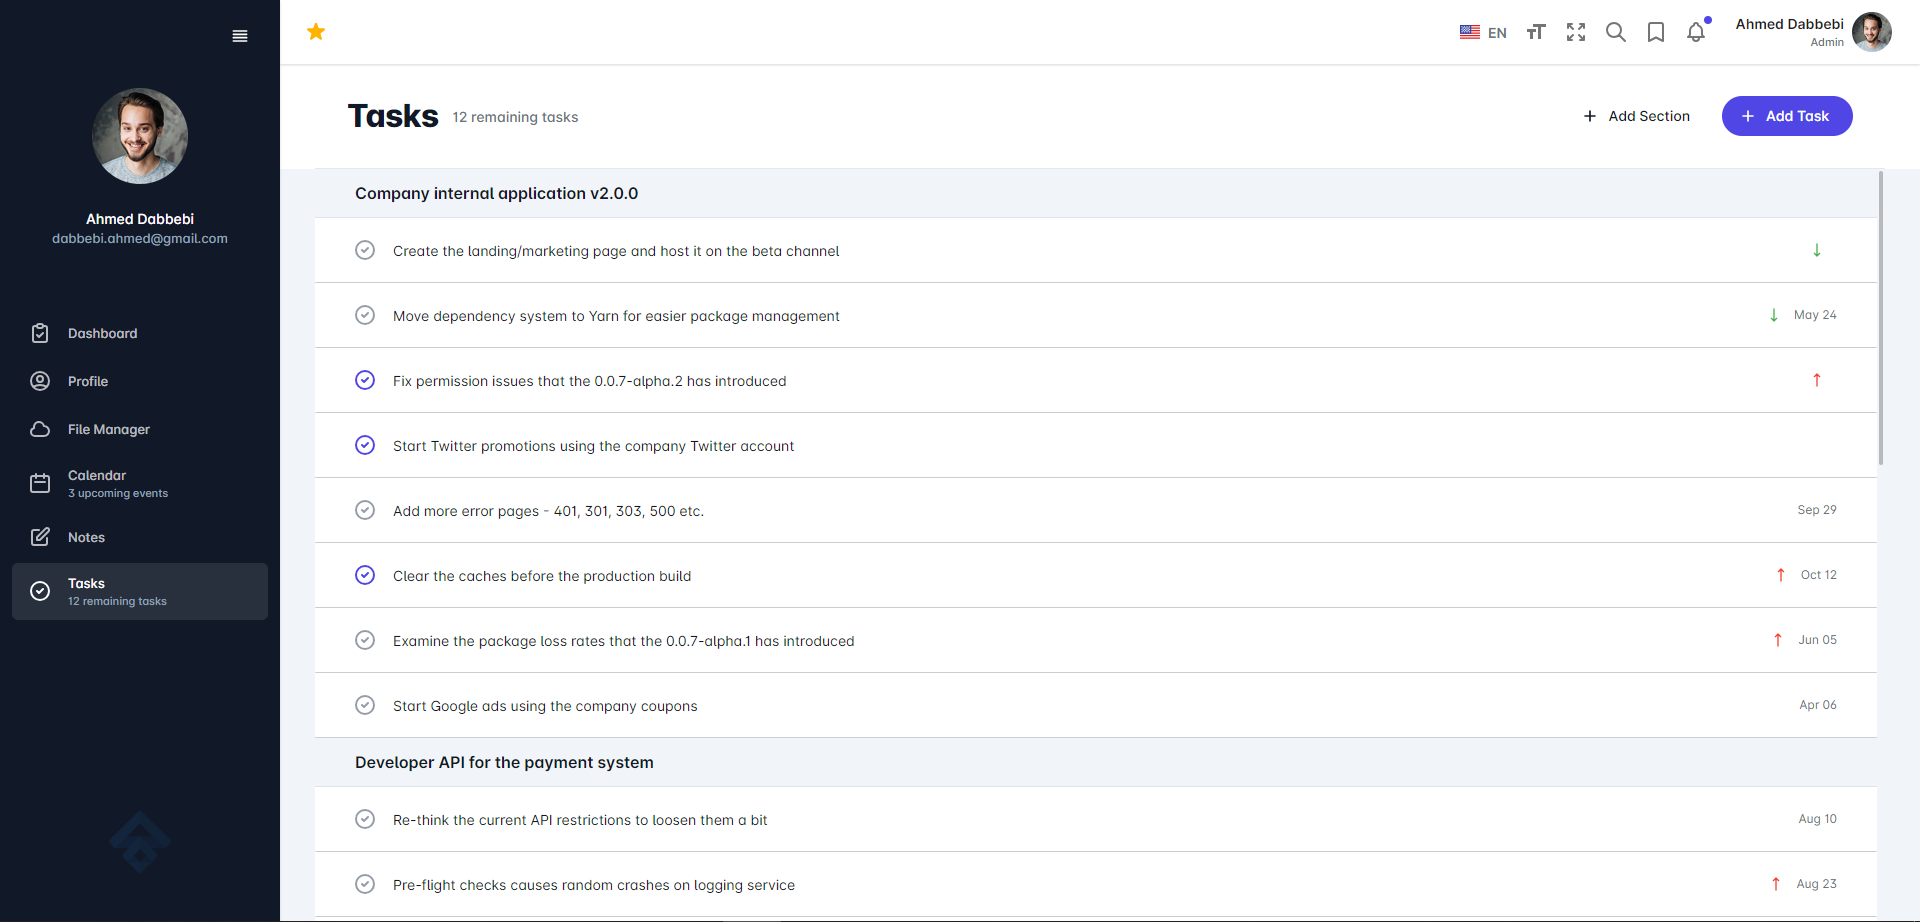
\includegraphics[scale=0.45]{chapitre4/interfaces/taches.PNG}
  \caption{Interface de tâches}   
  \label{fig:taches}
\end{figure}
\begin{figure}[H]
  \centering
  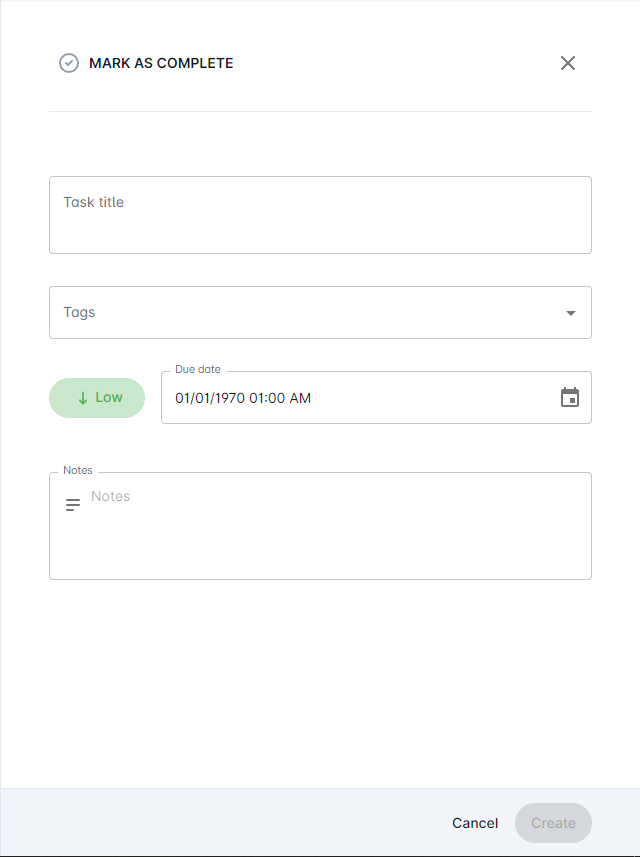
\includegraphics[scale=0.8]{chapitre4/interfaces/add task.PNG}
  \caption{Interface d'ajout d'une nouvelle tâche}   
  \label{fig:addtask}
\end{figure}
\begin{figure}[H]
  \centering
  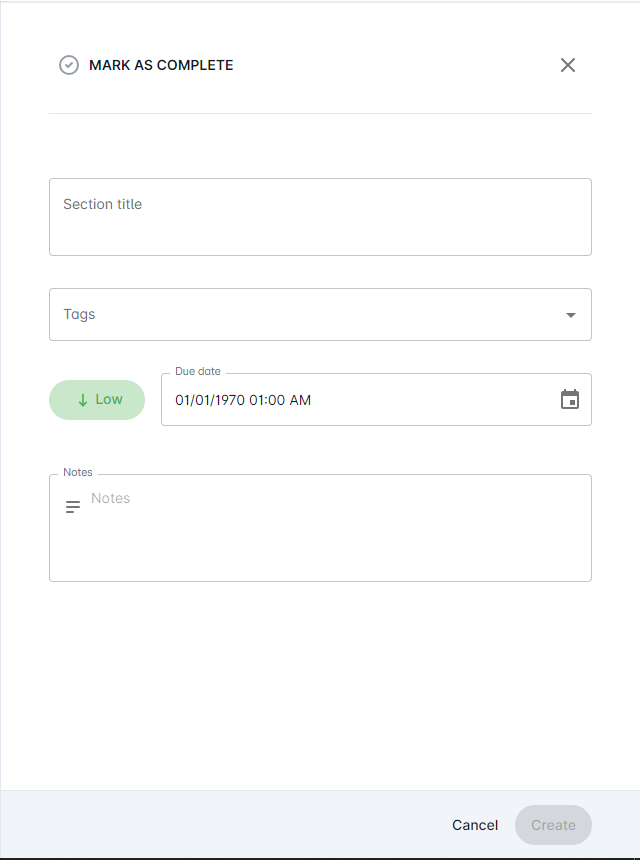
\includegraphics[scale=0.8]{chapitre4/interfaces/add section.PNG}
  \caption{Interface d'ajout d'une nouvelle section}   
  \label{fig:addsection}
\end{figure}


\vspace{5mm}
\section{Présentation de la partie IA}
\vspace{5mm}
\subsubsection{Objectif de l'algorithme d'IA }
\vspace{5mm}
L'algorithme d'IA vise à associer automatiquement un document PDF à un nom de matière spécifique parmi une liste de matières prédéfinis. Cela permet aux étudiants de catégoriser facilement leurs documents en fonction des matières étudiées, facilitant ainsi l'organisation et la gestion des fichiers académiques.

\vspace{5mm}
\subsubsection{Étapes principales de l'algorithme }
\vspace{5mm}
\begin{enumerate}

\item \textbf{ Extraction du texte }
\begin{itemize}[label=$\bullet$]
\item L'algorithme initie le processus en extrayant soigneusement le contenu du document PDF, préservant ainsi les nuances et les détails essentiels pour une analyse précise.
\end{itemize}
\vspace{3mm}
\item  \textbf{Nettoyage du texte }
\begin{itemize}[label=$\bullet$]
\item Le contenu extrait est soumis à un traitement méticuleux visant à éliminer non seulement les caractères inutiles, mais aussi à normaliser le texte, garantissant ainsi une cohérence et une clarté optimales.
\end{itemize}
\vspace{3mm}

\item  \textbf{Tokenisation }
\begin{itemize}[label=$\bullet$]
\item Une fois nettoyé, le texte est méticuleusement segmenté en mots ou en tokens, une étape fondamentale qui prépare le terrain pour une analyse exhaustive.
\end{itemize}
\vspace{3mm}

\item  \textbf{Vectorisation TF-IDF }
\begin{itemize}[label=$\bullet$]
\item Les tokens sont alors transformés en vecteurs numériques grâce à la technique sophistiquée de pondération TF-IDF. Cette méthode, tenant compte à la fois de la fréquence du terme et de son importance dans le contexte global du document, garantit une représentation fidèle et significative du contenu.
\end{itemize}
\vspace{3mm}

\item  \textbf{Calcul de similarité }
\begin{itemize}[label=$\bullet$]
\item À l'aide de la mesure de similarité cosinus, l'algorithme évalue avec rigueur la similitude entre le contenu du document et chaque sujet pertinent, offrant ainsi une perspective approfondie sur les relations sémantiques.

\end{itemize}
\vspace{3mm}

\item  \textbf{Détermination de la similarité maximale :}
\begin{itemize}[label=$\bullet$]
\item Guidé par une logique analytique, l'algorithme identifie avec précision la similitude la plus élevée parmi toutes les valeurs calculées, mettant en évidence la correspondance la plus pertinente entre le document et les sujets étudiés.
\end{itemize}
\vspace{3mm}

\item  \textbf{Association au sujet }
\begin{itemize}[label=$\bullet$]
\item En appliquant un seuil de similitude préétabli (tel que 0.2), l'algorithme attribue le document au sujet correspondant si la similitude dépasse ce seuil critique. Dans le cas contraire, le sujet est catégorisé comme "Inconnu", offrant ainsi une transparence et une granularité cruciales dans l'analyse des résultats.
\end{itemize}

\end{enumerate}

\vspace{8mm}
\subsubsection{Pseudo-code de l'algorithme }

\begin{figure}[H]
  \centering
  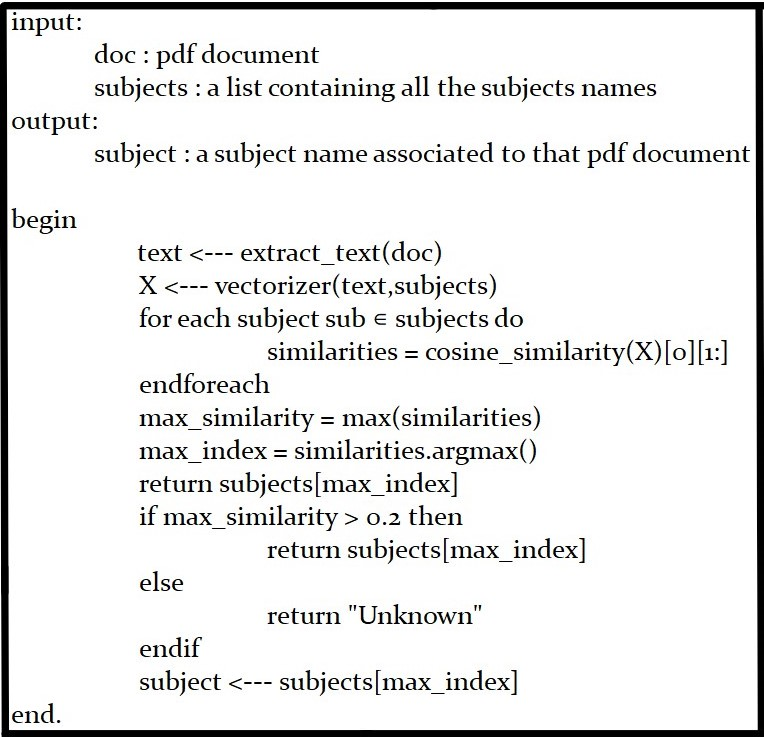
\includegraphics[scale=0.8]{chapitre4/algorithmqsqsqsq.jpg}
  \caption{Algorithme d'association de matière }   
  \label{fig:algorithm}
\end{figure}
\newpage
Cet organigramme \ref{fig:process} représente visuellement le fonctionnement de l'algorithme d'IA
\vspace{8mm}
\begin{figure}[H]
  \centering
  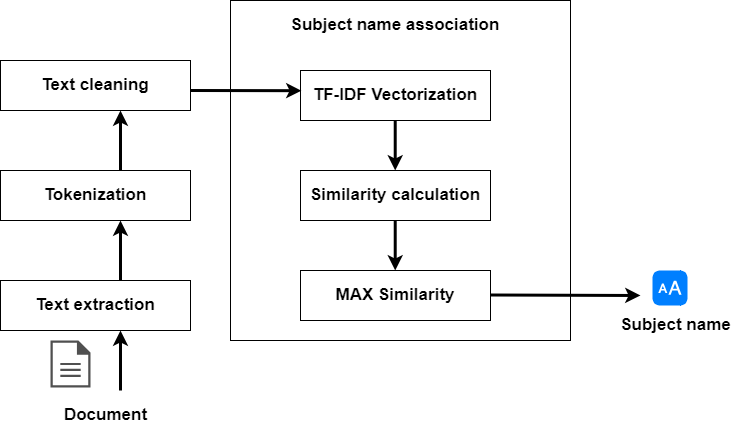
\includegraphics[scale=0.7]{chapitre4/general process.png}
  \caption{Processus général de notre solution proposée}   
  \label{fig:process}
\end{figure}
\vspace{10mm}
\subsubsection{Explication des avantages de l'IA dans votre application : }
L'intégration de l'IA dans notre plateforme web offre plusieurs avantages spécifiques 
\vspace{4mm}
\begin{itemize}[label=$\bullet$]
\item \textbf{Gestion simplifiée des études :} Catégorisation automatique des documents par sujet, ce qui permet une organisation plus efficace des ressources académiques et une réduction significative du temps passé à rechercher des informations pertinentes.
\vspace{3mm}
\item \textbf{Organisation automatisée :} Facilitation de la recherche et du tri des fichiers grâce à des algorithmes avancés de classification et de filtrage, rendant les documents facilement accessibles et consultables.
\vspace{4mm}
\item \textbf{Optimisation du calendrier et des tâches :} Meilleure gestion du temps et des priorités académiques, avec des suggestions personnalisées pour la planification des révisions et des échéances, contribuant ainsi à une organisation personnelle plus structurée et productive.
\vspace{4mm}
\item \textbf{Amélioration continue : } L’algorithme d’IA est conçu pour évoluer constamment, en apprenant des interactions des utilisateurs et des nouvelles données, ce qui enrichit l’application web et offre une expérience utilisateur de plus en plus pertinente et personnalisée aux étudiants.
\vspace{4mm}
\item \textbf{Support multilingue :} Capacité à traiter et à comprendre plusieurs langues, ce qui permet une utilisation plus inclusive et accessible de la plateforme par des étudiants de différentes régions et cultures.
\vspace{4mm}
\item \textbf{Analyse prédictive :} Utilisation de modèles prédictifs pour anticiper les besoins académiques et proposer des contenus et des ressources adaptés, facilitant ainsi l'apprentissage proactif et ciblé.
\end{itemize}
\vspace{8mm}

Grâce à ces innovations, notre plateforme devient un outil indispensable pour les étudiants, leur offrant non seulement une aide précieuse dans leurs études mais aussi une optimisation de leur temps et de leurs efforts, tout en s’adaptant continuellement à leurs besoins spécifiques.
\newpage

\section{Conclusion}
Dans ce chapitre, nous avons identifié les logiciels et les techniques que nous avons utilisées
durant la phase de développement de notre plateforme.\\ Puis, nous avons enrichi notre travail
par des imprimes écrans englobant la majorité des\\ fonctionnalités. \\
Enfin, nous avons exposé la partie IA sous forme d'un algorithme simplifié et un organigramme qui représente le fonctionnement de l'algorithme visuellement.







